\section{Breakdown of costs}

\begin{figure}[H]
    \centering
    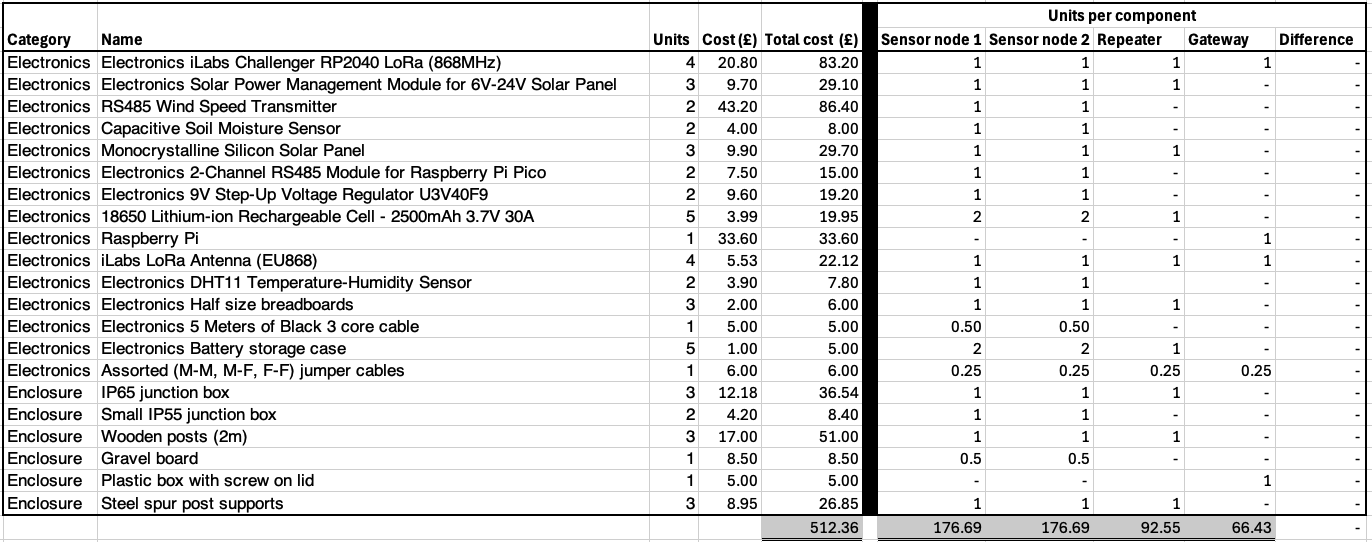
\includegraphics[width=0.9\textwidth]{contents/appendix/fig5/table.jpg}
    \caption{Table of component costs}
    \label{fig:cost-table}
\end{figure}

\begin{figure}[H]
    \centering
    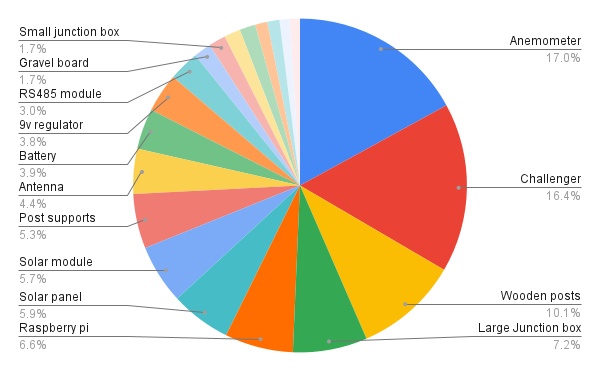
\includegraphics[width=0.8\textwidth]{contents/appendix/fig5/chart.png}
    \caption{Chart to visualise relative cost of components}
    \label{fig:cost-chart}
\end{figure}

\section{Interview excerpt with Small Brook Farms owners}\label{sec:small-brook-interview}

Interviewer: So you would need a weather station to observe very local weather, I expect.
What you're saying is that the BBC website weather is not necessarily relevant
to you?

Speaker 1: No, No , so there's another site which is in Sanford and we can have
conversations - we're what? - 5 miles apart 10 miles? 

Speaker 2: Yeah. So the other side of that hill there like a mile away you get a
different sort of weather, but even on this side of the [apple orchard] as
opposed to that side of the [apple orchard] like the wind can be less than
whatever else, its very localised. But you know you if you then go on that side
of the valley, it doesn't rain on this side. So like to be actually useful,
yeah, [weather monitoring] sort of has to be [based on] the farm.